\subsection{Coordinate vectors}

For example, the basis of $xy$ plane can be:

\[\mathfrak{B}=\left\{\begin{bmatrix} 1\\1\\0\\ \end{bmatrix}, \begin{bmatrix}1\\-1\\0\\ \end{bmatrix}\right\}\]

To form $\begin{bmatrix}1\\ 0\\0\end{bmatrix}$ with this basis, can do $\begin{bmatrix} 1\\0\\0\\ \end{bmatrix}=\frac{1}{2}\begin{bmatrix} 1\\1\\0\\ \end{bmatrix}+\frac{1}{2}\begin{bmatrix}1\\-1\\0\\ \end{bmatrix}$.
The coefficients used form the following vector:

\[\begin{bmatrix}\frac{1}{2}\\ \frac{1}{2}\end{bmatrix}\]

Known as \textbf{$\mathfrak{B}$-coordinate vector}.
Notation:

\[\left[\begin{bmatrix} 1 \\ 0 \\ 0 \end{bmatrix} \right]_\mathfrak{B}=\begin{bmatrix} \frac{1}{2} \\ \frac{1}{2} \\ \end{bmatrix} \]

\begin{framed}
\noindent
Generally, given $\mathfrak{B}=\left\{ \tb v_1, \tb v_2, \tb v_3, \dots, \tb v_m \right\}\subset \mathbb{R}^n$
is linearly independent, then $[\tb{v}_i]_{\mathfrak{B}}=\tb{e}_i\in\R^m$.
\end{framed}

This is because row-reducing the matrix of $\mathfrak{B}$ gives $\mathrm{rref}(A)$ where $A$ is this matrix. Given the same
$\mathfrak{B}$, can find the components of $\tb{w}$:

\[\left[\tb w \right]_\mathfrak{B}=\begin{bmatrix}c_1\\c_2\\ \vdots\\ c_m\end{bmatrix}\]
\[\tb{w}=c_{1} \tb{v}_{1}+c_{2} \tb{v}_{2}+\cdots+c_{m} \tb{v}_{m}\]

Thus,

\[\tb w = \begin{bmatrix}|&|&\dots&|\\ \tb v_1 &\tb v_2 & \dots &\tb v_m\\  |&|&\dots&| \end{bmatrix}\begin{bmatrix}c_1\\c_2\\\vdots\\c_m\end{bmatrix}\]

Matrix is called change of basis matrix $S$. A standard basis is given as $\tb{e}_1,\tb{e}_2,\cdots$. A nonstandard basis is not of this form.

\subsection{B-matrix}

If $A$ is $n\times n$ and $T(\tb{x})=A\tb{x}$ where $T:\R^n\rightarrow \R^n$, then there exists a matrix $B$ such that
$\left[T(\tb x)\right]_\mathfrak{B}=B\left[\tb x\right]_\mathfrak{B}$. This is called the $\mathfrak{B}-matrix$.
If $\tb{v}_i\in \mathfrak{B}$, then $[\tb{v}_i]_\mathfrak{B}=\tb{e}_i$.\\

\noindent
This means that 
$\left[T(\tb v_i)\right]_\mathfrak{B}=B\left[\tb v_i \right]_\mathfrak{B}=B\tb e_i$, so 
\textbf{the $i^{\mathrm{th}}$column of $B$ must be $[T(\tb{v}_i)]_\mathfrak{B}$}.\\

\noindent
Multiple ways to calculate $\mathfrak{B}$-matrix of $T$, considering $T$ to be a projection
onto $y=\frac{x}{3}$:

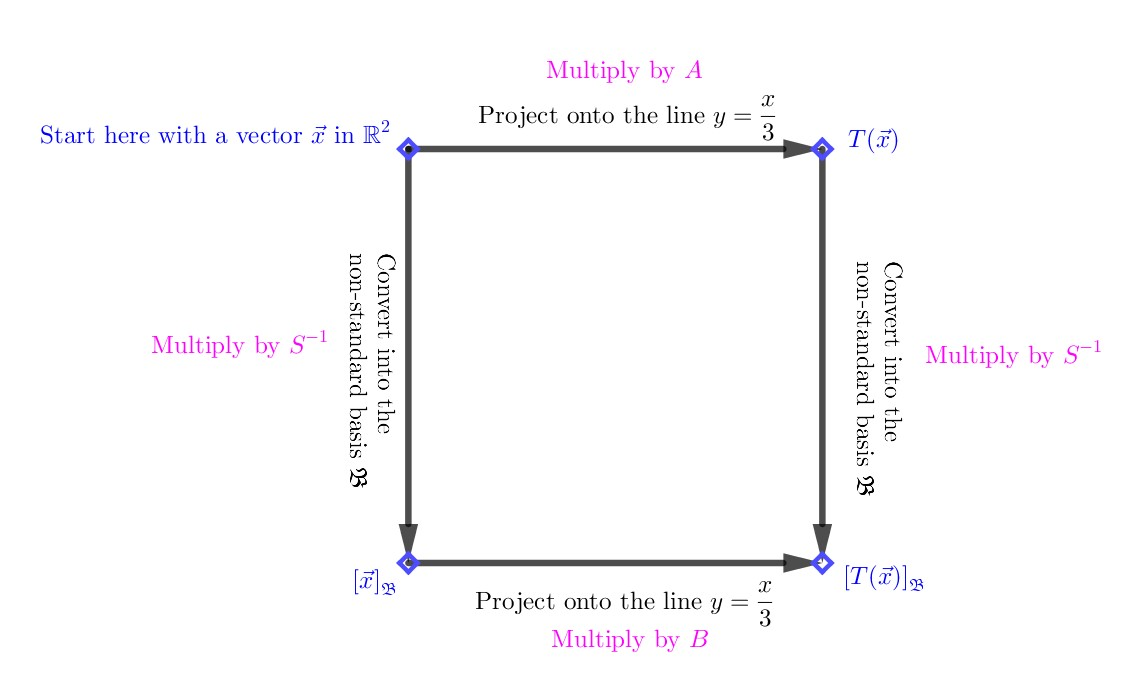
\includegraphics[scale=0.5]{CommutativeDiagram2.jpg}

Means that multiple ways to get to $[T(\tb{x})]_\mathfrak{B}$.
When following $\tb{x}$ and going right and down:

\[S^{-1}\left(A\tb x\right)=S^{-1}A\tb x=\left[T(\tb x) \right]_\mathfrak{B}\]

Going down and right:

\[B\left(S^{-1}\tb x\right)=BS^{-1} \tb x=\left[T(\tb x )\right]_\mathfrak{B}\]

Thus,

\begin{align*}
S^{-1}A=BS^{-1}\\
\boxed{S^{-1}AS=B}
\end{align*}

If this is satisfied, then $A$ is similar to $B$ or $A\sim B$.